\chapter{Background}\label{background}
\section{Neural Networks}
A neural network is a machine learning tool ideal for conducting supervised learning. As a relatively recent field, the application of neural networks has rapidly extended across many domains, such as  facial recognition at Facebook \cite{deepface}, translation for Microsoft \cite{translation}, spam filters for Google's Gmail \cite{gmail} and more. As such, it continues to be a hot topic in today's world of research.

\subsection{The Neuron}
The \textit{neuron} is the basic computational unit of a neural network. A \textit{layer} is comprised of one or more neurons. The computation performed by a neuron is shown below.
\begin{align}
\text{net} &= \mathbf{w \cdot x} + b\label{eq2.1}\\
y &= f(\text{net})
\end{align}
The \textit{fan-in} to a neuron is the amount of elements in the input vector $\mathbf{x} = x_1, x_2, \ldots, x_n$. For each element, there is a corresponding parameter referred to as a \textit{weight}. The weights of a neuron form the weight vector $\mathbf{w}$. The neuron also has an offset $b$ which helps with normalization. The neuron's net is first computed as shown in equation \ref{eq2.1}, and then the output, or activation, is computed according to the neuron's activation function. This is shown visually in figure \ref{neuron}.
\begin{figure}
	\centering
	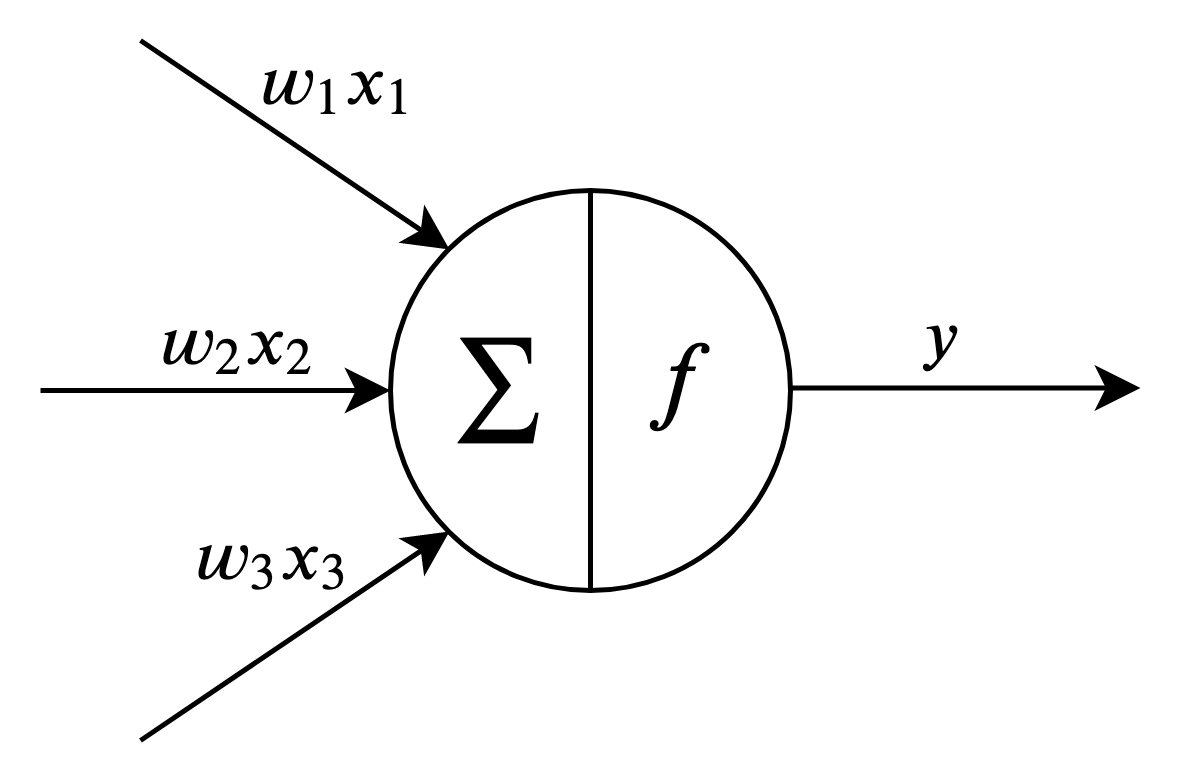
\includegraphics[width=2in]{figures/neuron}
	\caption{A neuron with 3 inputs; bias term omitted for simplicity.}\label{neuron}
\end{figure}

\paragraph{Weight Initialization}
Proper weight initialization is paramount to successfully training a neural network. Firstly, weights cannot be all initialized to 0, for this will result in the same gradient for all weights, and thus all weights will be updated in the same manner. This would effectively mean that the network would become a function of a singular weight.

The most na\"ive way to initialize weights would to assign each weight a random value between some range. In most cases, this is good enough for the network to converge to a relatively optimal solution so long as the range is not to extreme. A recent popular and effective way to initialize the weights is through He Initialization, which randomly initializes weights using a normal distribution with a mean of 0 and a variance of $\frac{2}{\text{fan\_in}}$ \cite{HeZR015}. 


\subsection{Fully-Connected Layers}
A fully-connected layer is a vector of neurons. All neurons in a fully-connected layer receive the same input vector. This vector is the previous layer's output. A fully-connected layer with 3 neurons receiving input from an input layer is shown in figure \ref{fully-connected}. The output is a vector comprising of the outputs of each neuron. Each neuron output is calculated using the $M$-sized input vector as shown in equation \ref{n-act} and added to output vector $\mathbf{y}$.
\begin{align}
y_i &= f_{\text{act}}\left( b + \sum_{j=1}^{M}(w_jx_j) \right) \label{n-act} \\
\mathbf{y} &= \left\{ y_1, y_2, \ldots, y_n \right\} 
\end{align}

\begin{figure}
	\centering
	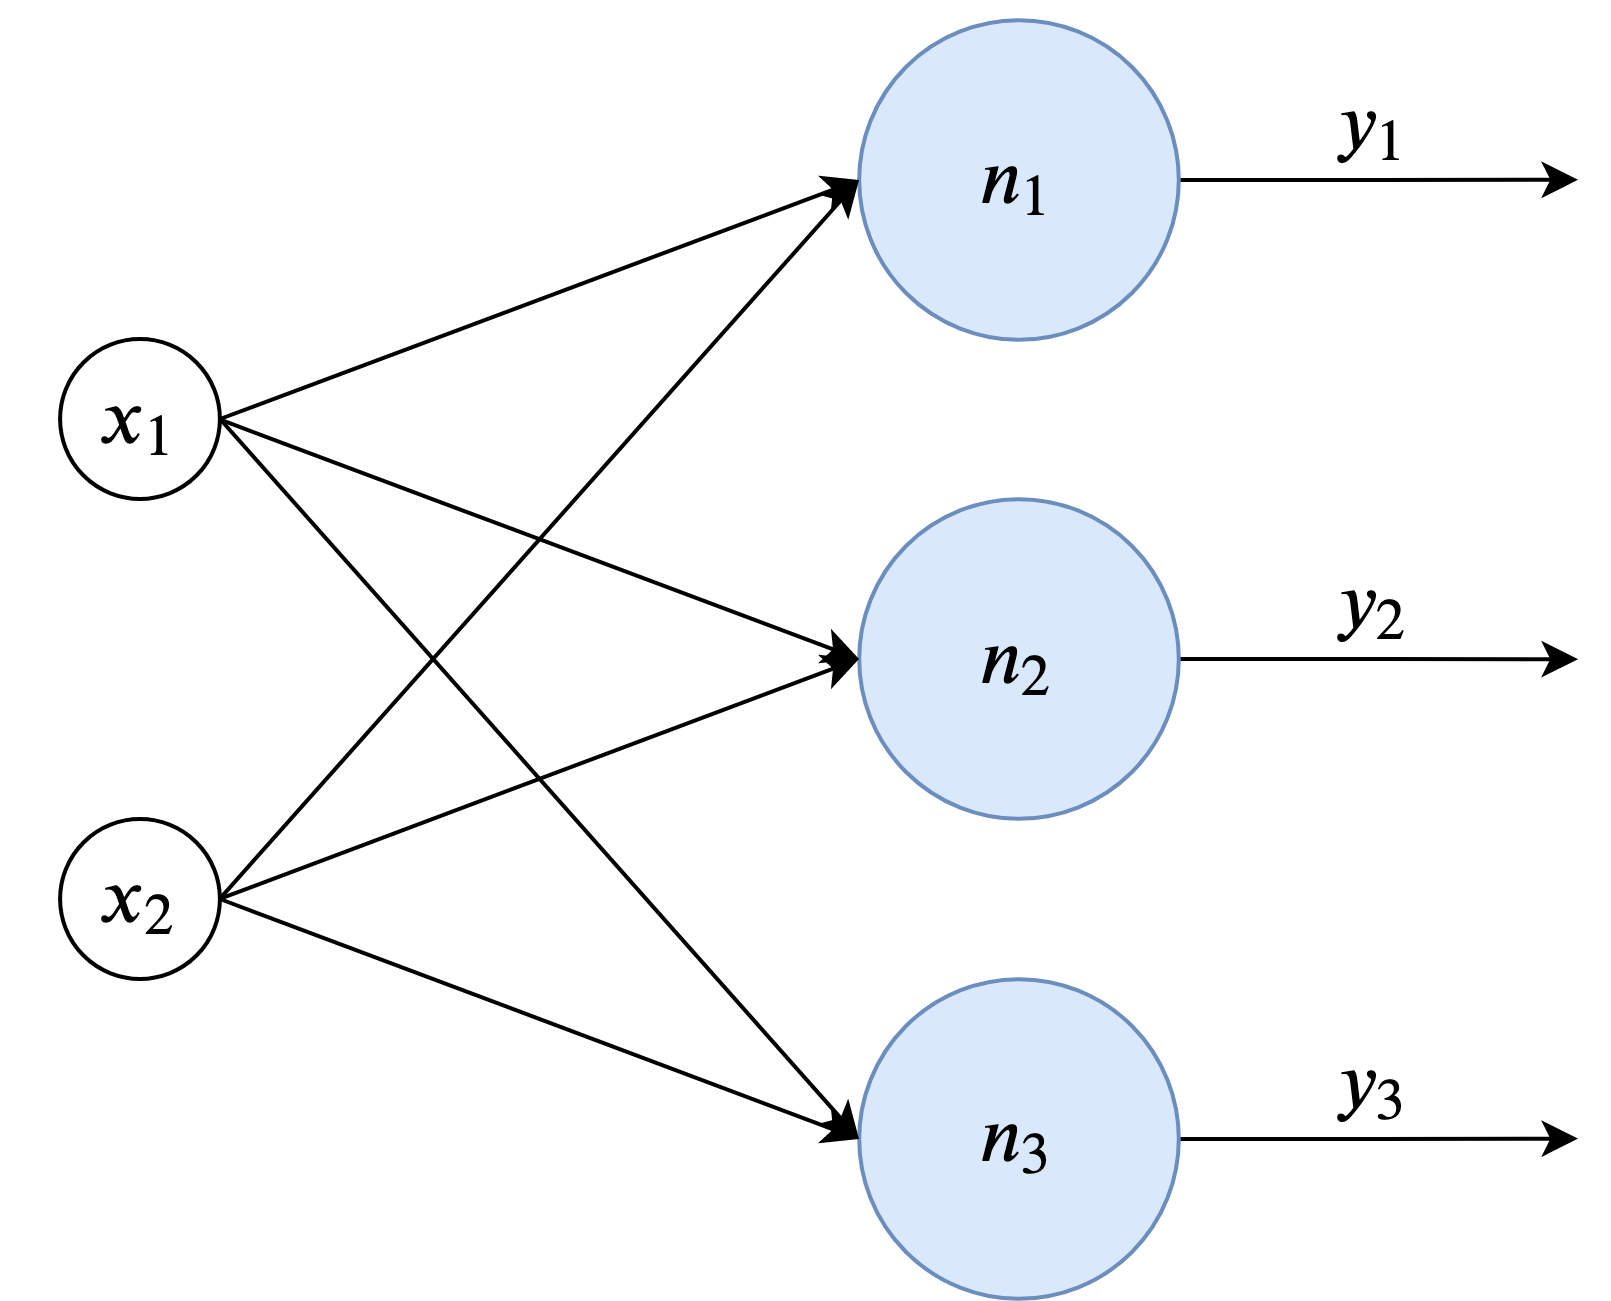
\includegraphics[width=3in]{figures/fully-connected}
	\caption{A fully-connected layer with 3 neurons, each receiving an input vector of size 2 from the input layer.}\label{fully-connected}
\end{figure}

\subsection{Activation Functions}
Without activation functions, the neural network would simply devolve to a linear classifier. Activation functions provide neural networks with the non-linearity to solve complex classification problems. Two of the most common activation functions are the rectified linear unit (ReLU) and the softmax function. These are the two activation functions that were chosen to be used in the software and hardware models of this thesis.

\paragraph{ReLU}
ReLU is a powerful activation function that has found widespread use due to its mathematical simplicity. The ReLU function is shown in equation \ref{relu-func}.
\begin{align}
y = \max(0, x) \label{relu-func}
\end{align}
Notably, the ReLU function is much easier to compute compare to the sigmoid or hyperbolic tangent functions, which both use the exponential function. The ReLU function also quite frequently performs just as well if not better compared to other activation functions. One of the reasons is because it does not suffer as much from the vanishing gradient problem \cite{pmlr-v15-glorot11a}. The vanishing gradient problem is encountered during training using backpropagation, which uses the chain rule from calculus, briefly covered in section \ref{backprop}. Since gradients will always be less than 1 for most loss functions, the gradients become geometrically smaller with each layer. Since ReLU only saturates in one direction, ReLU networks will be more sparse, in the sense that many of the neurons will have an output of 0. 

ReLU-based neural networks also tend to reach convergence quicker than neural networks using the sigmoid or the hyperbolic tangent functions. It also results in a sparsely activated network, in that since the neuron output is 0 if the net is negative, that many neurons in the network will have an output of 0. This is also similar to how biological neurons also follow a sparse firing model, and has shown to be effective \cite{pmlr-v15-glorot11a}. 

Conversely, since active neurons in ReLU network are sparse, this brings rise to another potential problem, the ``Dying ReLU Problem.'' This problem occurs when the sparsity increases to the point where a large majority of the neurons in the network become inactive during training and ultimately never become active again. Fortunately, this problem can be ameliorated with proper weight initialization \cite{Lu2019DyingRA}.

\paragraph{Softmax}
The softmax function converts a vector of logits to a vector of probabilities. It has seen widespread use in neural networks that are used to predict the class of an input. The softmax function is shown in equation \ref{sm-func}.
\begin{align}
\sigma(\mathbf{x})_i = \frac{e^{x_i}}{\Sigma_{j=1}^C e^{x_j}} \label{sm-func}
\end{align}
In this function, $x_i$ is the net of neuron $i$ from the layer. Generally, the softmax function is used in the last layer to generate probabilities for multi-class problems. Each neuron in the layer represents a class, so the size of the last layer is equivalent to the number of classes, $C$. In much of the literature, the softmax portion of a neural network is referred to as the softmax layer as opposed to simply being the activation function of the neuron nets in the last layer.


\subsection{Cross-Entropy Loss}
Cross-entropy loss is a probabilistic loss function and as such, is frequently paired with the softmax activation function. This allows for the probabilities output from the softmax function to be used as inputs for calculating the cross-entropy loss. Cross-entropy loss is computed using probabilities and is shown in equation \ref{cel-eq}.
\begin{align}
\mathcal{L}(\mathbf{x}) = \sum_{i=1}^{N} q(x_i)\log(p(x_i))\label{cel-eq}
\end{align}
In this function, $q(x_i)$ is the true probability of $x$ belonging to class $i$, therefore, $q(x_i) = 1$ when $x$ is of class $i$ and $0$ otherwise; $p(x_i)$ is equal to the predicted probability.

\subsection{Backpropagation}\label{backprop}
Backpropagation is a method in which the weights of a network can be trained on a dataset by propagating the loss (also referred to as gradient in gradient descent) from the output layer backward through the network. There are three computational steps to be made during backpropagation: propagating loss gradients to the previous layer, using loss gradients for neurons in a layer to calculate individual weight gradients, and then finally to update the weights.

\paragraph{Calculating the Loss Gradients in the Output Layer}
For the first part of backpropagation, we must use the partial derivative of the loss function with respect to each of the neuron outputs to begin backpropagation. Note that the cross-entropy loss is calculated directly from the probabilities from the softmax function of the last layer. Therefore, the loss must derive the loss function with respect to the probabilities, and then must derive the softmax function in order to attain $\frac{\delta \mathcal{L}}{\delta \text{net}_o}$ for the neurons in the last layer. The calculus is omitted for brevity, but the final result is clean and simple, as shown in equation \ref{sm-deriv} \cite{sm-derivative}. 
\begin{align}
\frac{\delta \mathcal{L}}{\delta \text{net}_{o,i}} &= p_i - y_i	\label{sm-deriv}
\end{align}
This equation calculates the partial derivative of the loss with respect to the net of the last layers output neuron. $p_i$ is the probability computed from the softmax function and $y_i$ is the true probability. Thus, if the input sample belong to class $i$, $y_i$ is equal to 1, otherwise $y_i$ is 0. Once the initial gradient for each neuron in the last layer has been calculated, backpropagation of the loss through the previous layers is possible.

\paragraph{Backpropagating the Loss Gradient}
The strength of backpropagation is being able to use the chain rule to calculate gradients from previous layers. At a high-level, a neuron in a previous layer's output will affect the nets of neurons in the next layer. Since each activation is multiplied by a weight, the affect on the net is determined by a weight. For example, if a neuron's activation $a_o$ increases by $\epsilon$, then each of the next layer's neuron nets will increase by $w\times \epsilon$, where $w$ is the weight for that connection. This connection is also somtimes referred to as a \textit{synapse}, a term inspired from neuroscience.

An example illustrating this is shown in figure \ref{neuron-bp}. The gradients for the nets of $C$, $D$, and $E$ are represented by $\delta$. The gradient of a net is commonly referred to as the \textit{sensitivity} of a neuron. Subsequently, the weights on the synapses are also shown. With this knowledge, we can calculate $\frac{\delta \mathcal{L}}{\delta B}$ as shown in equation \ref{ex-nbp}.
\begin{align}
\frac{\delta \mathcal{L}}{\delta B} = \delta_cw_{(b,c)} + \delta_dw_{(b,d)} + \delta_ew_{(b,e)} \label{ex-nbp}
\end{align}
\begin{figure}
	\centering 
	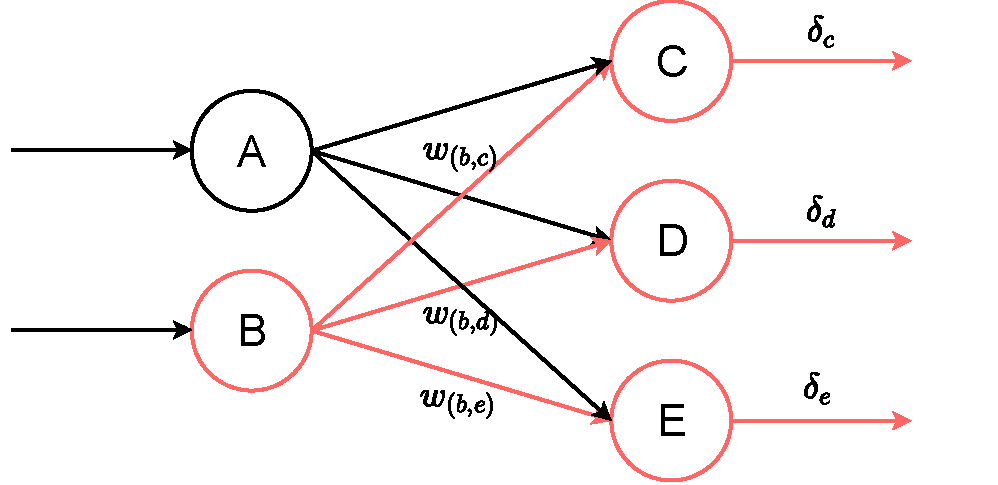
\includegraphics[width=\textwidth]{figures/neuron_bp.pdf}
	\caption{Example of backpropagating the loss gradient to the previous layer. Values used in backpropagating the loss to neuron B shown in red.} \label{neuron-bp}
\end{figure}

In more formal mathematical terms, if we know the $\frac{\delta \mathcal{L}}{\delta \text{net}}$, or $\delta$, for each neuron in a layer with $n$ neurons, then we can calculate the gradient for any neuron $i$'s activation in the previous layer containing $m$ neurons as shown in equation \ref{nbp-eq}.
\begin{align}
\frac{\delta \mathcal{L}}{\delta m_i} = \sum_{j=1}^{n} \delta_jw_{(i,j)} \label{nbp-eq}
\end{align}

The sensitivity for the neurons in layer $m$ can then be computed using the derivative of the activation function. Since this thesis only uses ReLU, the derivative is simple to calculated and shown in equation \ref{deriv-relu}. Note that the ReLU derivative is undefined at 0, however, in practical cases using a derivative of 0 works fine.
\begin{align}
f'(x) = \begin{cases}
	1 & x > 0\\
	0 & x < 0\\
	\text{undefined} & x = 0
\end{cases}\label{deriv-relu}
\end{align}


\paragraph{Calculating Weight Gradients}
Once the sensitivity $\delta$ of neuron is known, calculating the gradients of individual weights and biases is possible. From a high-level, if we increase weight $w$ by $\epsilon$, then the product term of the net for the neuron will be $(w + \epsilon)a_i$, a net increase of $a_i\times\epsilon$. Therefore, the gradient for a weight is dependent on how large the weight's corresponding activation is. That means the weight corresponding to a large activation will have a much larger gradient than a weight corresponding to a small activation.

Returning to the previous example, the figure has now been updated to show how weight gradients for neuron $C$, this is shown in figure \ref{weight-bp}. The gradients for the 2 connecting weights are calculated as shown below. $A_o$ and $B_o$ are the activations of neuron $A$ and $B$, respectively. As one would expect, the gradient of a weight is dependent on the magnitude of the neuron activation it is multiplied with, and the sensitivity of the neuron whose net it is summed with.
\begin{align*}
\frac{\delta \mathcal{L}}{\delta w_{(a,c)}} &= \delta_cA_o\\
\frac{\delta \mathcal{L}}{\delta w_{(b,c)}} &= \delta_cB_o
\end{align*}
\begin{figure}
	\centering 
	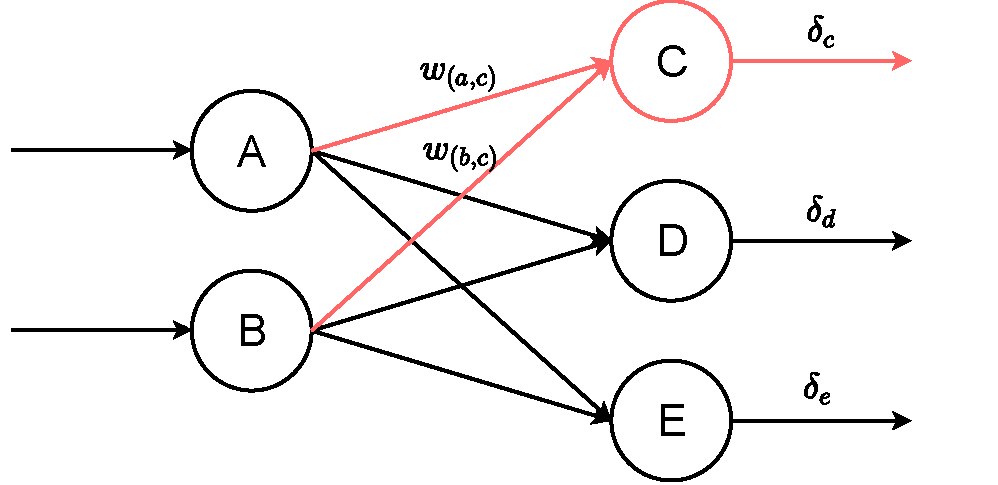
\includegraphics[width=\textwidth]{figures/weight_bp.pdf}
	\caption{Example of computing weight gradients. Relevant values shown in red.} \label{weight-bp}
\end{figure}

\paragraph{Updating the Weights}
Once $\frac{\delta \mathcal{L}}{\delta w}$ is known for every single weight, the final step of backpropagation is to update the weights. This is performed by scaling the gradient for the weight by a value, known as the learning rate, $\eta$, and then subtracting it from the weight, since this will move the weight in the direction that lowers the loss. This is shown in equation \ref{weight-update}.
\begin{align}
	w_{new} = w_{old} - \eta\frac{\delta \mathcal{L}}{\delta w} \label{weight-update}
\end{align}



\subsection{Hyperparameters}
There are many hyperparameters to consider when designing a neural network. As described in section \ref{backprop}, the learning rate determines how of an impact the loss gradient has when updating the weight. Related to the learning rate is another hyperparameter known as momentum. The term is inspired from physics and has the effect of incorporating past updates in a geometrically decreasing fashion. We first define a few parameters:
\begin{center}
	\begin{tabular} {r l}
		$m$  \hspace{12pt}---& the momentum parameter\\ 
		$v$  \hspace{12pt}---& `velocity' \\
		$\eta$ \hspace{12pt}---& the learning rate \\
		$dw$ \hspace{12pt}---& the loss gradient for some weight or bias $w$. 
	\end{tabular}
\end{center}The momentum-based update can then be mathematically represented in the following manner:
\begin{align*}
v &=  (m \times v) - (\eta \times w) \\
w &= w + v 
\end{align*}
Each time each time we update $w$, previous updates update will also have an effect. A typical value for momentum is 0.9.

The final hyperparameter to be discussed in this section is batch size. Batch size determines the amount of forward and backward passes should be computed before performing a weight update. There is no typical value for the batch size and the optimal batch sizes varies largely by dataset and problem type.

\section{Deep-Learning Frameworks}
Deep-learning has come into the spotlight in the past few years and as such, many popular and robust frameworks have been developed. Some of the most popular frameworks are TensorFlow which is developed by Google, and PyTorch which is developed by Facebook. Other popular frameworks include Keras and Caffe. These frameworks are generally relatively simple to use while delivering high performance. 


\subsection{PyTorch}
For this thesis, PyTorch has been chosen as the framework to construct a model against which to benchmark my results. PyTorch offers a simplistic interface to build highly customizable neural networks. In addition, it also has support for GPU-training, thus both CPU and GPU benchmarks can be obtained.

\section{Related Work}
With the surge in popularity of neural networks, there has been a lot of research focusing on improving the performance of inference and training. Zhao et al. developed a data-streaming solution (F-CNN) using an FPGA to perform 32-bit floating point training and inference. They used a CPU to communicate weights, addresses, and training data over a PCI-E bus, ultimately obtaining roughly a 4 times speedup over a CPU implementation and a 7.5 times more power-efficient compared to a GPU implementation \cite{FCNN}.

The Alternative Computing Technologies lab at the  Georgia Institute of Technology has begun promising work on a framework called TABLA, that generates FPGA code for a multitude of machine learning models. The framework is based on creating individual processing engines inside processing units and thus creating a more generalized design by having schedulers assign work to these processing units. Training and inference have been tested with promising results on a Xilinx Zynq-7000 SoC and the group are aiming to make it public in the near future \cite{TABLA}.

The majority of work based on accelerators for neural networks has been focused on inference. Google's Tensor Processing Unit (TPU) has found real-world success by performing inference on networks using Google's TensorFlow Lite framework \cite{TPU}. This framework sacrifices precision for speed and obtains great performance with little punishment to overall accuracy, due to inference being less accuracy reliant than training. The Eyeriss is another hardware accelerator chip that has been developed to improve inference. It is designed by the Eyeriss Project team at the Massachusetts Institute of Technology. Its primary contribution is a novel dataflow optimization for convolutional neural networks called RS, for row stationary. This optimization allows for a high percentage of data reuse during inference \cite{eyeriss}.

The overwhelming majority of research regarding hardware acceleration for neural networks is focused on inference. Consequently, aside from the aformentioned F-CNN FPGA-based framework for training neural network, there has not been much research investigating neural network training on an FPGA. This work differs from the F-CNN as it investigates the effectiveness of using fixed-point arithmetic instead of floating point during training, allowing for extra speed at the sacrifice of accuracy. Furthermore, this work proposes that the main advantage of using a training accelerator is for datasets that train optimally with smaller batch sizes.

\todo[inline]{Perhaps make use of Courbariaux: Results from Courbariaux et al. show that training has much stricter accuracy requirements than inference.}